\setmainfont{Noteworthy}
%TODO: provide your details here.
\begin{frame}
    \frametitle{About Your Fellows}
    \begin{itemize}
        \item Hi there! We are \textcolor{blue}{\textbf{ Khadijah Farooqi}  \textcolor{black}{and}\textbf{ Abdullah Salman}}.
        \item We are Associate Students at ITU.
    \end{itemize}
\end{frame}

\begin{frame}
    \frametitle{Recap of the prev lecture}
    \vspace{0.3cm} % Adds spacing for better visual appearance
    \begin{itemize}
        \item \textbf{Problem:} \textcolor{red}{Find the k\textsuperscript{th} smallest element in an array with distinct elements.}
        \vspace{0.3cm} % Adds spacing between items
        \item \textcolor{blue}{\textbf{Algorithm: \textcolor{teal}{Guess Select Algorithm }}}
        \vspace{0.2cm} % Adds spacing before the sub-item list
        \begin{itemize}
            \item \textcolor{black}{\textbf{Input:} Array \textit{A} and \textit{k}, where \textit{k} is the position of the desired element.}
            \item \textcolor{black}{Uniformly Randomly pick a number g GUESS as an element from \textit{A}.}
            \item \textcolor{black}{Partition \textit{A} into:}
            \begin{itemize}
                \item \textit{L}: Elements less than \textit{g}.
                \item \textit{R}: Elements greater than \textit{g}.
            \end{itemize}
            \item \textcolor{black}{Compute the rank of \textit{g} using \textit{L} and \textit{R}.}
            \item \textcolor{black}{If $|L| = k-1$, return \textit{g}.}
            \item \textcolor{black}{Else if $|L| > k-1$, recursively select \textit{k\textsuperscript{th}} element from \textit{L}.}
            \item \textcolor{black}{Otherwise, recursively select \textit{(k - |L| - 1)\textsuperscript{th}} element from \textit{R}.}
        \end{itemize}
    \end{itemize}
    \vspace{0.5cm} % Adds spacing at the bottom of the slide for a clean look

    
\end{frame}

\begin{frame}
    \frametitle{Recap of the prev lecture}
    \vspace{0.3cm} % Adds spacing for better visual appearance
    \begin{itemize}
        \item \textbf{Problem:} \textcolor{red}{Find the k\textsuperscript{th} largest element in an array with distinct elements.}
        \vspace{0.3cm} % Adds spacing between items
        \vspace{0.2cm} % Adds spacing before the sub-item list
        \begin{itemize}
            \item \textcolor{blue}{\textbf{Method 1: Swap the Definition of L and R}}
            \begin{itemize}
                \item \textit{L}: Elements greater than  \textit{g}.
                \item \textit{R}: Elements smaller than \textit{g}.
                \item Now repeat the same guess algorithm stated above to find the k\textsuperscript{th} largest element.
            \end{itemize}
            \vspace{0.3cm}
            \item \textcolor{blue}{\textbf{Method 2: Transforming k}}
            \begin{itemize}
                \item Let $k = n - k$ and use the selection process for this adjusted \textit{k}.
            \end{itemize}
        \end{itemize}
    \end{itemize}
    \vspace{0.5cm} % Adds spacing at the bottom of the slide for a clean look
\end{frame}



\begin{frame}
    \frametitle{Convex Function}
    \vspace{0.3cm} % Adds spacing for better visual balance

    A function \( f : \mathbb{R}^{n} \to \mathbb{R} \) is convex if its domain is a convex set and for all \( x, y \) in its domain, and all \( \lambda \in [0, 1] \), we have:

    \[
    f( \lambda x +(1 - \lambda)y) \leq \lambda f (x) + (1 -\lambda )f(y)
    \]

    \begin{minipage}{0.48\linewidth}
        \centering
        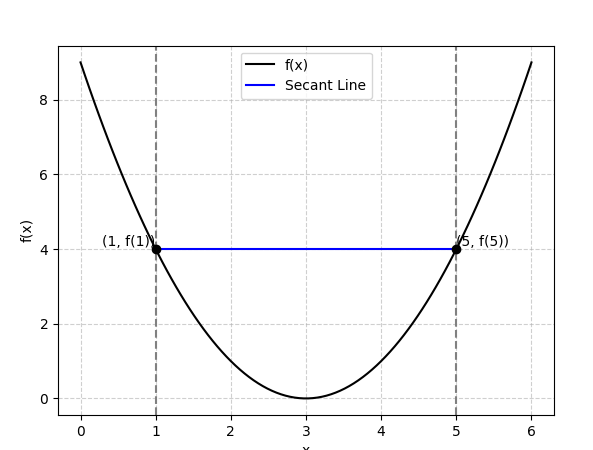
\includegraphics[width=\linewidth]{graph.png} % Ensure the image fits
    \end{minipage}%
    \hfill
    \begin{minipage}{0.48\linewidth}
    \begin{block}{\textcolor{DarkCyan}{Relation to Digression}}
        \small % Makes the text smaller
        The term Digression refers to the \textcolor{purple}{deviation from the straight-line connection}. \\
        \textcolor{orange}{->} A \textcolor{purple}{convex function} digresses \textcolor{purple}{downward} from the secant line. \\
        \textcolor{orange}{->} A \textcolor{purple}{linear function} shows \textcolor{purple}{no digression}. \\
        \textcolor{orange}{->} A \textcolor{purple}{concave function} digresses \textcolor{purple}{upward} from the secant line.
        \end{block}
    \end{minipage}


    \vspace{0.5cm} % Adds spacing at the bottom of the slide for a clean look
\end{frame}


\begin{frame}
    \frametitle{Facts About Convex Functions}
    \vspace{0.3cm}

    \begin{itemize}
        \item The sum of two convex functions is also convex. If \( g(x) \) and \( f(x) \) are convex, then \( r(x) = g(x) + f(x) \) is also convex.
        \item Geometrically, the line segment connecting \( (x, f(x)) \) to \( (y, f(y)) \) lies above the graph of \( f \).
        \item If \( f \) is continuous, checking convexity for a fixed \( \lambda \in (0,1) \), such as \( \lambda = \frac{1}{2} \), is sufficient.
        \item A function \( f \) is concave if \( -f \) is convex.
    \end{itemize}


\begin{center}
        \textit{\textcolor{gray}{}}
    \end{center}
\end{frame}

\begin{frame}
    \frametitle{Examples of Convex Functions}
    \vspace{0.3cm}

    \textbf{Examples of Univariate Convex Functions:}
    \begin{itemize}
        \item \( e^{ax} \)
        \item \( -\log(x) \)
        \item \( x^a \) (defined on \( \mathbb{R}_{++} \)), for \( a \geq 1 \) or \( a \leq 0 \)
        \item \( -x^a \) (defined on \( \mathbb{R}_{++} \)), for \( 0 \leq a \leq 1 \)
        \item \( |x|^a \), for \( a \geq 1 \)
        \item \( x \log(x) \) (defined on \( \mathbb{R}_{++} \))
    \end{itemize}

    \vspace{0.3cm}

    Reference: S. Boyd and L. Vandenberghe, \textit{Convex Optimization}, Cambridge University Press, 2004. Available at: \url{http://stanford.edu/~boyd/cvxbook/}
\end{frame}



% \begin{frame}
%     \frametitle{Digersion-Convex Function}
%     \vspace{0.4cm} % Adds spacing for better visual balance
    
%     \begin{itemize}
%        In words, this means that if we take any two points x and y, then f evaluated at any convex combination of these two points should be no larger than the same convex combination of f(x) and f(y).
%     \end{itemize}
%     \vspace{0.4cm} % Adds spacing between the block and the list

    
    
%     \vspace{0.5cm} % Adds spacing at the bottom of the slide for a clean, symmetrical appearance
    
% \end{frame}




\begin{frame}
\frametitle{Convex Theorem}
\begin{block}{Definition}
    A function \( f(x) \) is \textbf{convex} if it satisfies the inequality:
    \[ f(\lambda x + (1 - \lambda)y) \leq \lambda f(x) + (1 - \lambda) f(y) \]
    for all \( x, y \) in its domain and \( \lambda \in [0,1] \).
\end{block}

\vspace{0.5cm}
\begin{block}{Importance}
    The convex function theorem plays an important role in:
    \begin{itemize}
        \item Dynamic Programming
        \item Divide and Conquer
        \item Optimization Problems
    \end{itemize}
\end{block}
\end{frame}

\begin{frame}
\frametitle{Proof of Convex Theorem}
    \textcolor{blue}{Using the Convex Theorem: }
    \[ f (\lambda a + (1 − \lambda)b) \leq \lambda f (a) + (1 − \lambda)f (b).
    \]
    \textcolor{blue}{\textbf{Let's Take:}}
    \[
        \lambda = \frac{a}{a+b}, \quad (1-\lambda) = \frac{b}{a+b}
    \]
    \textcolor{blue}{\textbf{Why Choosing} \( \lambda = \frac{a}{a+b} \) \textbf{and} \( (1-\lambda) = \frac{b}{a+b} \):} \\
    \vspace{10pt} 
    Its because \( \lambda \) must satisfy \( \lambda \in [0,1] \) and \( \lambda + (1−\lambda) = 1 \), \\
    \vspace{10pt} 
    so, taking \( \lambda = \frac{a}{a+b} \) and \( (1-\lambda) = \frac{b}{a+b} \) ensures that \( \lambda \) 
    and \( 1−\lambda \) are positive and sum to 1. \\
    \textcolor{purple}{\[
    \lambda + (1-\lambda) = \frac{a}{a+b} + \frac{b}{a+b} = \frac{a+b}{a+b} = 1
    \]}

\end{frame}

\begin{frame}
\frametitle{Proof of Convex Theorem}

    \textcolor{blue}{Substituting \( \lambda = \frac{a}{a+b} \) and \( (1-\lambda) = \frac{b}{a+b} \), we get:}
    \[
    f \left( \frac{a}{a+b} a + \frac{b}{a+b} b \right) \leq \frac{a}{a+b} f(a) + \frac{b}{a+b} f(b)
    \]
    \textcolor{blue}{Simplifying the left-hand side:}
    \[
    f \left( \frac{a^2+b^2}{a+b} \right) \leq \frac{a f(a) + b f(b)}{a+b}
    \]
\end{frame}

\begin{frame}
\frametitle{Example: Quadratic Function}
\begin{block}{Function Choice}
    Let \( f(x) = x^2 \) (a convex function). Choose \( a = 2 \), \( b = 4 \).
\end{block}

\begin{block}{Applying Convexity}
    \begin{align*}
    \lambda &= \frac{2}{2+4} = \frac{1}{3}, \quad 1 - \lambda = \frac{4}{6} = \frac{2}{3} \\
    \lambda a + (1-\lambda)b &= \frac{1}{3} (2) + \frac{2}{3} (4) = \frac{10}{3}
    \end{align*}
    
    Checking convexity inequality:
    \[ f\left(\frac{10}{3}\right) \leq \frac{1}{3} f(2) + \frac{2}{3} f(4) \]
\end{block}
\end{frame}

\begin{frame}
\frametitle{Example: Quadratic Function (Continued)}
\begin{block}{Simplification}
    Substituting \( f(x) = x^2 \):
    \[ \left(\frac{10}{3}\right)^2 \leq \frac{1}{3} (4) + \frac{2}{3} (16) \]
    
    Simplifying,
    \[ \frac{100}{9} \leq 12 \]
\end{block}

\begin{block}{Conclusion}
    Since \( \frac{100}{9} \approx 11.11 \leq 12 \), the inequality holds, confirming the convexity of \( f(x) = x^2 \).
\end{block}
\end{frame}


\begin{frame}{Mathematical Induction (Revision)}
    \large\textcolor{blue}{Climbing a Infinite Ladder: }\\ 
     \vspace{0.4cm}
     \small
    Suppose that we have an infinite ladder,
    we want to know whether we can reach
    every step on this ladder. We know two
    things :\\
     \vspace{0.4cm}
    \textcolor{DarkCyan}{a) We can reach the first step of the ladder.}\\
    \textcolor{DarkCyan}{b) If we can reach a particular step of the ladder,
    then we can reach the next step.}\\
    Induction says that these two pieces of
    information enough to reach the required
    conclusion!\\
    \begin{block}{Here is how it works (informally!)}
        From \textcolor{red}{(a)} we can reach the first step. Then by applying \textcolor{red}{(b)} we can reach the second step. Applying \textcolor{red}{(b)} again, the third step.
        And so on. We can apply \textcolor{red}{(b)} any number of times to reach any
        particular step, no matter how high up.\\
         \vspace{0.2cm}
        After \textcolor{red}{100} uses of \textcolor{red}{(b)}, we know that we can
        reach the \textcolor{red}{101st} step.
    \end{block}
    
\end{frame}
    
\begin{frame}{Principal of Mathematical Induction (Revision)}
    \large
    To prove that P(n) is true for all positive integers n, we complete
    these steps:
    \small
    \colorbox{orange}{Basis Step: Show that P(1) is true.}\\
    \colorbox{orange}{Inductive hypotheis: We asume that statement is true for some positive integer k}\\
    
    \colorbox{orange}{Inductive Step(proof): Based on the assumption, we prove that the
    statement must be true for k + 1}
    \large
    To complete the inductive step, assuming the inductive hypothesis
    that P(k) holds for an arbitrary integer k, show that must P(k + 1)
    be true.
\end{frame}

\begin{frame}{Proof by Induction: Example (Revision)}
    \begin{figure}
        
        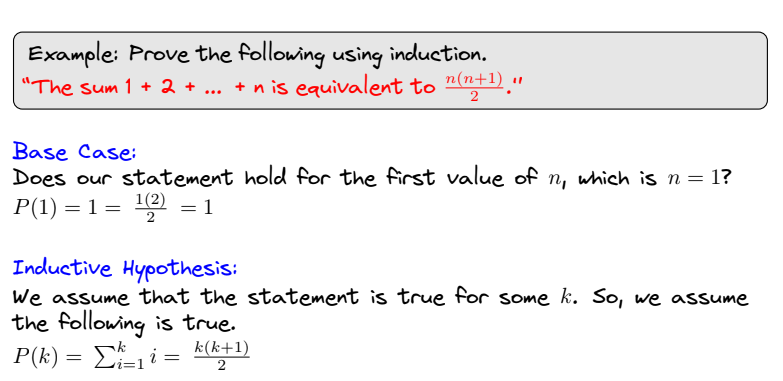
\includegraphics[width=0.9\linewidth]{Selection_844.png}
        % \caption{Example from Discrete Structure Course}
        \label{fig:enter-label}
    \end{figure}
    \small
    Reference: Professor's DS slides of F2023
\end{frame}

\begin{frame}{Proof by Induction: Example (Revision)}
    \begin{figure}
        \centering
        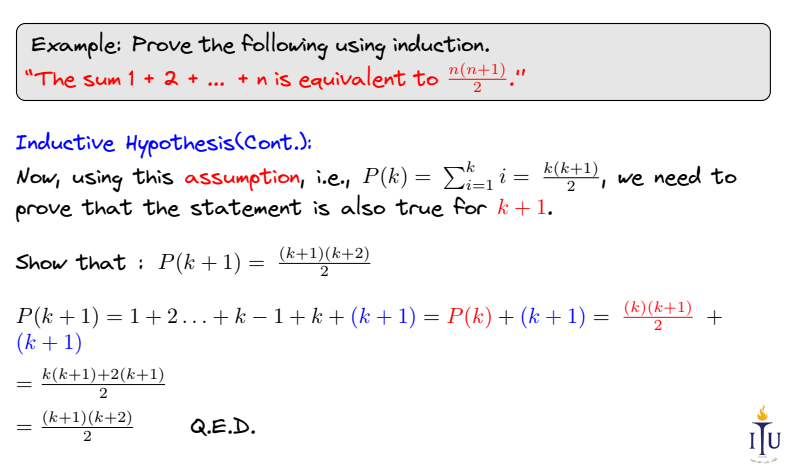
\includegraphics[width=0.9\linewidth]{image2.png}
        % \caption{Enter Caption}
        \label{fig:enter-label}
    \end{figure}
    \small
    Reference: Professor's DS slides of F2023
\end{frame}

\begin{frame}
    \frametitle{Recursion}
    \vspace{0.4cm} % Adds spacing for better visual balance
        \textcolor{DarkCyan}{Recursion} is a method to \textcolor{red}{solve a problem} where the solution \textcolor{red}{depends on solutions to smaller subproblems} of the same problem. Recursive functions (function calling itself) are used to solve problems based on Recursion. The main challenge with recursion is to \textcolor{red}{find the time complexity of the Recursive function}.
    \vspace{0.4cm}
    \begin{block}{\textcolor{blue}{Methods of Solving Recursion}}
    \end{block}
    \vspace{0.4cm} % Adds spacing between the block and the explanation

    \begin{itemize}
        \item Tree Method
        \vspace{0.3cm} % Adds spacing between items for readability
        \item Substitution Method
        \vspace{0.3cm}
        \item Master Theorem
    \end{itemize}
    
    \vspace{0.5cm} % Adds spacing at the bottom for a clean look
\end{frame}


\begin{frame}
    \frametitle{Recursion}
    \begin{block}
       {\textcolor{blue}{The Recursion-Tree Method $\rightarrow$ \textcolor{DarkCyan}{useful for guessing the asymptotic bound of a recurrence relation}.}}
    \end{block}
    
    \vspace{0.5cm} % Adds spacing at the bottom for a clean look
\end{frame}

\begin{frame}{Recurrence - Recursion Tree Relationship}
\begin{figure}
    \centering
    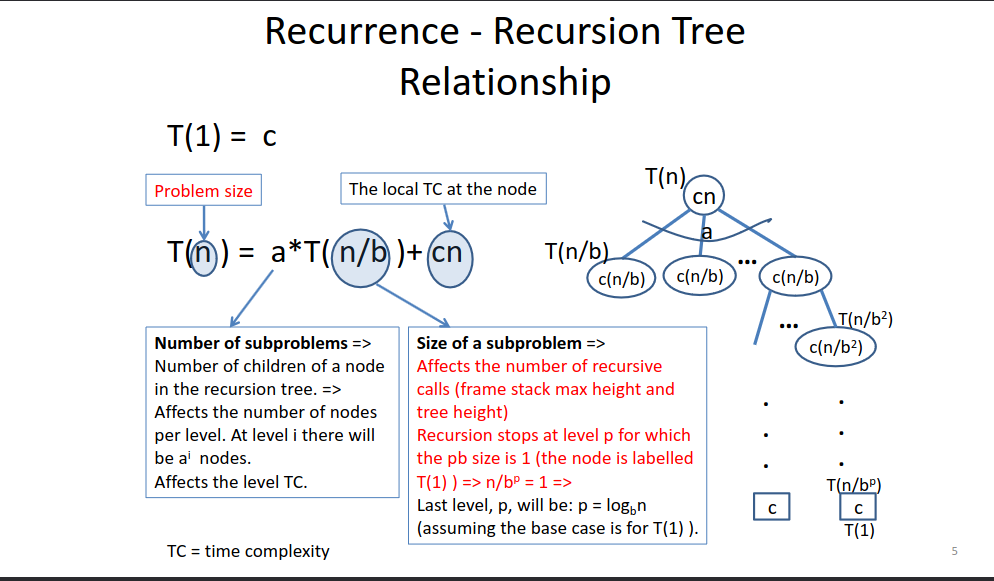
\includegraphics[width=0.8\linewidth]{Selection_856.png}
    % \caption{Enter Caption}
    \label{fig:enter-label}
    
\end{figure}
\small
    Reference: \href{https://ranger.uta.edu/~alex/courses/3318/lectures/08_recurrences.pdf}{https://ranger.uta.edu/~alex/courses/3318/lectures/08recurrences.pdf}
\end{frame}

\begin{frame}{Recursion Tree Method}
    
    \small

    \textbf{\textcolor{blue}{Recurrence Relation:}}
    \small
    \[
    T(n) = 2T\left(\frac{n}{2}\right) + c
    \]
    \textbf{\textcolor{blue}{Base Case:}}
    \[
    T(1) = c
    \]

    \textbf{\textcolor{blue}{Recursion Tree:}}
    \small
    \begin{itemize}
        \item At each level, the problem size halves (in this case).
        \item Number of nodes doubles at each level.
        \item Level \( p \) has \( 2^p \) nodes, each with problem size \( \frac{n}{2^p} \).
        \item Recursion stops when problem size is 1:
        \[
        \frac{n}{2^p} = 1 \Rightarrow p = \lg n
        \]
    \end{itemize}
    \textbf{\textcolor{blue}{Total Time Complexity:}}
    \[
    \text{Total TC} = c(1 + 2 + 4 + \dots + 2^p) = c \cdot (2^{p+1} - 1) = 2c \cdot 2^p = 2cn = \Theta(n)
    \]
\end{frame}


\begin{frame}{Recursion Tree for \( T(n) = 2T(n/2) + c \)}
    \textbf{Recursion Tree:}
    \scriptsize % Smaller font size for better fit
    \tiny
    \begin{center}
        \begin{forest}
            for tree={
                grow=south, % Tree grows top to bottom
                parent anchor=south, % Parent node connects to the bottom
                child anchor=north,  % Child node connects to the top
                align=center,
                s sep=0.3cm, % Vertical spacing between levels
                l sep=0.2cm % Horizontal spacing between nodes
            }
            [\( T(n) \)
                [\( T(n/2) \)
                    [\( T(n/4) \)
                        [\( T(n/8) \)
                            [\( \vdots \)
                                [\( T(1) \), edge=dashed]
                            ]
                            [\( T(1) \), edge=dashed]
                        ]
                        [\( T(n/8) \)
                            [\( T(1) \), edge=dashed]
                            [\( \vdots \)
                                [\( T(1) \), edge=dashed]
                            ]
                        ]
                    ]
                    [\( T(n/4) \)
                        [\( T(n/8) \)
                            [\( T(1) \), edge=dashed]
                            [\( \vdots \)
                                [\( T(1) \), edge=dashed]
                            ]
                        ]
                        [\( T(n/8) \)
                            [\( \vdots \)
                                [\( T(1) \), edge=dashed]
                            ]
                            [\( T(1) \), edge=dashed]
                        ]
                    ]
                ]
                [\( T(n/2) \)
                    [\( T(n/4) \)
                        [\( T(n/8) \)
                            [\( T(1) \), edge=dashed]
                            [\( \vdots \)
                                [\( T(1) \), edge=dashed]
                            ]
                        ]
                        [\( T(n/8) \)
                            [\( \vdots \)
                                [\( T(1) \), edge=dashed]
                            ]
                            [\( T(1) \), edge=dashed]
                        ]
                    ]
                    [\( T(n/4) \)
                        [\( T(n/8) \)
                            [\( T(1) \), edge=dashed]
                            [\( \vdots \)
                                [\( T(1) \), edge=dashed]
                            ]
                        ]
                        [\( T(n/8) \)
                            [\( \vdots \)
                                [\( T(1) \), edge=dashed]
                            ]
                            [\( T(1) \), edge=dashed]
                        ]
                    ]
                ]
            ]
        \end{forest}
    \end{center}
\end{frame}


% ---- Slide 2: Table and Complexity Analysis ----
\begin{frame}{Tree Method - Complexity Analysis}
    \textbf{Table Representation:}
    \begin{table}[]
        \centering
        \begin{tabular}{|c|c|c|c|c|}
            \hline
            \textbf{Level} & \textbf{Arg/pb size} & \textbf{TC of 1 node} & \textbf{Nodes per level} & \textbf{Level TC} \\
            \hline
            0 & \( n \) & \( c \) & 1 & \( c \) \\
            1 & \( n/2 \) & \( c \) & 2 & \( 2c \) \\
            2 & \( n/4 \) & \( c \) & 4 & \( 4c \) \\
            \(\vdots\) & \(\vdots\) & \(\vdots\) & \(\vdots\) & \(\vdots\) \\
            \( i \) & \( n/2^i \) & \( c \) & \( 2^i \) & \( 2^i c \) \\
            \hline
        \end{tabular}
    \end{table}

    \vspace{0.5cm}

    \textbf{Stopping Condition:}
    \[
    \frac{n}{2^p} = 1 \Rightarrow p = \log_2 n
    \]

    \vspace{0.5cm}

    \textbf{Total Tree Complexity:}
    \[
    \text{Tree TC} = c(1 + 2 + 2^2 + \dots + 2^p) = c \cdot \frac{2^{p+1} - 1}{2 - 1} = 2c \cdot 2^p = 2cn = \Theta(n)
    \]
\end{frame}

\begin{frame}{Tree Method - Reference Image}
 \begin{figure}
         \centering
         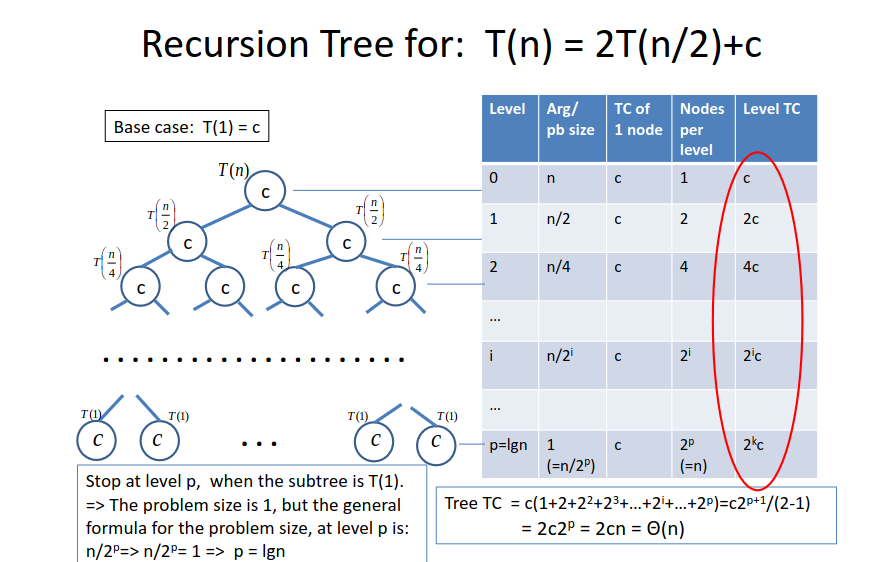
\includegraphics[width=0.8\linewidth]{treemethod.png}
         % \caption{Enter Caption}
         \label{fig:enter-label}
     \end{figure}    
     \small
    Reference: \href{https://ranger.uta.edu/~alex/courses/3318/lectures/08_recurrences.pdf}{https://ranger.uta.edu/~alex/courses/3318/lectures/08recurrences.pdf}
     
\end{frame}




\begin{frame}
    \frametitle{Recursion}
    \vspace{0.4cm} % Adds spacing for better visual balance
    \begin{block}{\textcolor{black}{Substitution - \textcolor{red}{The substitution method is a technique used to solve recurrence relations by guessing the form of the solution and then verifying it using mathematical induction.}}}
    \end{block}
    
    \vspace{0.5cm} % Adds spacing at the bottom for a clean look
\end{frame}




\begin{frame}
    \frametitle{Substitution}
    \vspace{0.4cm} % Adds spacing for better visual balance

    \begin{block}{\textcolor{red}{KEY CONCEPTS}}
    \end{block}
    \vspace{0.4cm} % Adds spacing between the block and the explanation

    \begin{itemize}
        \item Recursive Relation
        \vspace{0.3cm} % Adds spacing between items for readability
        \item Base case
        \vspace{0.3cm}
        \item Inductive Hypothesis
    \end{itemize}
    
    \vspace{0.5cm} % Adds spacing at the bottom for a clean look
\end{frame}



\begin{frame}
    \frametitle{Substitution}
    \vspace{0.4cm} % Adds spacing for better visual balance
    \begin{block}{\textcolor{black}{Recursive Relation\textcolor{red}{->An equation that recursively defines a sequence of values.}}}
    \end{block}
    \vspace{0.4cm}
    \begin{block}{\textcolor{black}{Base Case\textcolor{red}{->The condition under which the recursion stops.}}}
    \end{block}
    \vspace{0.4cm}
    \begin{block}{\textcolor{black}{Inductive Hypothesis\textcolor{red}{->An assumption that the solution holds for a smaller input.}}}
    \end{block}

    \vspace{0.5cm} % Adds spacing at the bottom for a clean look
\end{frame}



\begin{frame}
    \frametitle{Steps in Substitution Method}
    \vspace{0.4cm} % Adds spacing for better visual balance
    \begin{itemize}
        \item Guess the Form of the Solution: Make an educated guess about the form of the solution based on the recurrence relation.
        \vspace{0.3cm} % Adds spacing between items for readability
        \item Verify the Guess: Use mathematical induction to prove that the guessed solution is correct.
        \vspace{0.3cm}
        \item Solve for Constants: Determine the constants in the solution to match the initial conditions.
    \end{itemize}
    
    \vspace{0.5cm} % Adds spacing at the bottom for a clean look
\end{frame}



\begin{frame}
    \frametitle{Substitution - Example}
    \vspace{0.4cm} % Adds spacing for better visual balance
    \begin{itemize}
        \item Recurrence Relation: T(n) = 2T(n/2) + n
        \vspace{0.3cm} % Adds spacing between items for readability
        \item Guess: T(n) = O(n log n)
        \vspace{0.3cm}
        \item Verification: Use induction to prove that T(n) ≤ cn log n for some constant c.
    \end{itemize}
    
    \vspace{0.5cm} % Adds spacing at the bottom for a clean look
\end{frame}


\begin{frame}
    \frametitle{Substitution - Mathematical Induction}
    \vspace{0.4cm} % Adds spacing for better visual balance
    \begin{block}{\textcolor{black}{Base Case\textcolor{red}{->Show that the solution holds for the smallest value of n.}}}
For \( n = 1 \), 

\[
T(1) = 1 \leq c \cdot 1 \cdot \log 1
\]

    \end{block}
    \vspace{0.4cm}
    \begin{block}{\textcolor{black}{Inductive Step\textcolor{red}{->Assume the solution holds for n/2 and prove it holds for n.}}}
    \end{block}
    \vspace{0.4cm}
    \vspace{0.5cm} % Adds spacing at the bottom for a clean look
\end{frame}


% \begin{frame}
%     \frametitle{Recursion}
%     \vspace{0.4cm} % Adds spacing for better visual balance
%     \begin{block}{{\textcolor{red}{Mein sony ja rha ho }}}
%     \end{block}

%     \vspace{0.5cm} % Adds spacing at the bottom for a clean look
% \end{frame}

\begin{frame}
    \frametitle{Substitution- Common Mistakes}
    \vspace{0.4cm} % Adds spacing for better visual balance
     \begin{itemize}
        \item Incorrect Guesses: Choosing a form that does not satisfy the recurrence relation.
        \vspace{0.3cm} % Adds spacing between items for readability
        \item Insufficient Verification: Not fully proving the solution with induction.
        \vspace{0.3cm}
        \item Ignoring Base Cases: Failing to verify the base case in the induction process.
    \end{itemize}



    \vspace{0.5cm} % Adds spacing at the bottom for a clean look
\end{frame}



\begin{frame}
    \frametitle{Substitution- Application}
    \vspace{0.4cm} % Adds spacing for better visual balance
\begin{block}{\textcolor{black}{Merge Sort: \textcolor{red}{Analyzing the time complexity using the substitution method.}}}


    \end{block}
\begin{itemize}
    \item \textbf{Recurrence:}  
    \[
    T(n) = 2T(n/2) + n
    \]

    \item \textbf{Solution:}  
    \[
    T(n) = O(n \log n)
    \]
\end{itemize}

\begin{block}{\textcolor{black}{Quick Sort: \textcolor{red}{Understanding the worst-case and average-case scenarios.}}}


    \end{block}

\begin{itemize}
    \item \textbf{Recurrence:}  
    \[
    T(n) = T(k) + T(n - k - 1) + n
    \]
\item \textbf{Solution:}

O(nlogn) on average and in the best case, but 
O(n \textsuperscript{2}) in the worst case.



\end{itemize}






    % \vspace{0.5cm} % Adds spacing at the bottom for a clean look
\end{frame}





\begin{frame}{Recurrence Solving - Example no. 1}
    {Solving $T(n) = C + T(9n/10)$}
    \textbf{\textcolor{blue}{Using Tree Method:}}\\
    \vspace{0.2cm}
    \textbf{Expanding the recurrence:}
    \begin{align*}
        T(n) &= C + T(9n/10) \\
        T(9n/10) &= C + T((9/10)^2 n) \\
        T(n) &= C + \left( C + T((9/10)^2 n) \right) \\
              &= 2C + T((9/10)^2 n) \\
        T((9/10)^2 n) &= C + T((9/10)^3 n) \\
        T(n) &= 3C + T((9/10)^3 n)
    \end{align*}
    \textbf{Generalizing:}
    \begin{equation*}
        T(n) = iC + T((9/10)^i n)
    \end{equation*}
    % \textbf{Stopping Condition:} $(9/10)^i n = 1$ leads to $i = \log_{10/9} n$.
\end{frame}

\begin{frame}{Recurrence Solving - Example no. 1}
    {Solving $T(n) = C + T(9n/10)$}
    {Summing the Contributions}
    Each level contributes: $C(9/10)^i n$.
    \begin{equation*}
        T(n) = \sum_{i=0}^{\infty} C(9/10)^i n
    \end{equation*}
    This is a geometric series with sum:
    \begin{equation*}
        T(n) = C n \sum_{i=0}^{\infty} (9/10)^i
    \end{equation*}
    Using the formula for an infinite geometric series:
    \begin{equation*}
        \sum_{i=0}^{\infty} r^i = \frac{1}{1 - r}, \quad \text{where } r = 9/10,
    \end{equation*}
    we get:
    \begin{equation*}
        T(n) = C n \frac{1}{1 - 9/10} = C n \cdot 10.
    \end{equation*}
    \textbf{Final Result:} $T(n) = 10 C n$.
\end{frame}

\begin{frame}{Recurrence Solving - Example no. 1}
    {Solving $T(n) = C + T(9n/10)$}
    \textbf{\textcolor{blue}{Using Substitution Method:}}\\
    \vspace{0.2cm}
    
    We now have a guess: $T(n) \leq C \cdot 10 n$.\\
    \textbf{Defining the Constant:}
    \begin{equation*}
        T(n) \leq C a n, \quad \text{where } a \text{ is a constant } .
    \end{equation*}
    \textbf{Base Case:} For $n \leq 5$, we assume:
    \begin{equation*}
        T(n) \leq C a \cdot 5.
    \end{equation*}
    \textbf{Inductive Hypothesis:} Assuming it is true for all $k < n$, we prove it for $n$:
    \begin{equation*}
        Cn \left( 1 + \frac{9}{10} a \right) \leq Cna.
    \end{equation*}
\end{frame}

\begin{frame}
    \frametitle{Recurrence Solving - Example no. 1\\ \small {Solving $T(n) = C + T(9n/10)$}}
    
Proof:
    \[
    {T(n) \leq \text{Can}}
    \]
    \[ {T(n) = C.n +  T( \frac{9n}{10})}
    \]
    By inductive Hypothesis:
    \small
    \[
    = \text{C.n} + \frac{\cdot 9}{10} n \cdot Ca
    \]
    
    \[
    T(n) = \text{C.n}  \left(1 + \frac{9}{10} a\right)
    \]
    
    \[
    \text{C.n}\left(1 + \frac{9}{10} a\right) \leq \text{C.n.}a 
    \]
    
    \[
    1 + \frac{9}{10} a \leq a
    \]
    
    \[
    1 \leq a - \frac{9}{10} a
    \]
    
    \[
    1 \leq \frac{a}{10} \rightarrow       10 \leq a
    \]

\end{frame}

\begin{frame}
    \frametitle{Q/A}
    \vspace{0.4cm} % Adds spacing for better visual balance
    \begin{block}{\textcolor{black}{That's why we assume 10 as 'a' in first in substitution in the class}}
    \end{block}
  
    \textit{\textcolor{gray}{Ammar asked prof how did we replace 
    $T(n) = cn + T \left(\frac{9}{10} n\right)$ to $cn + \left(\frac{9}{10}\right) nca$}}

    \vspace{0.4cm}
    
    \textit{\textcolor{black}{Professor: We did this through Inductive Hypothesis}}
    
    \textcolor{gray}{Hamza asked prof about the sign in 
    $T(n) = cn \cdot \left(1 + \frac{9}{10} nca\right)$ that it should be less than or equal to ($\leq$).}

    \textit{\textcolor{black}{Hamza was right, and professor changed it to $T(n) \leq \text{Cn} + \frac{ 9}{10} n \cdot ca$}}
    
    \begin{block}{\textcolor{red}{If we change number of chunks what will happen??}}
    
    \textit{\textcolor{black}{Recurrence would change}}

    \end{block}
    
\end{frame}



\begin{frame}\frametitle{Recurrence Solving - Example no. 2\\ \small {Solving $T(n) = 2T(n/2) + Cn$}}
    \textbf{\textcolor{blue}{Guessing a Solution: }} \textcolor{black} { Assume $T(n) = a C n$.} \\[8pt]

    \textbf{\textcolor{blue}{Base Case: }} \textcolor{black}{ Same as before.} \\[8pt]

    \textbf{\textcolor{blue}{Inductive Hypothesis:   }} \textcolor{black} {Assume true for all $k < n$.} \\[8pt]


    \begin{align*}
        T(n) &= 2T(n/2) + Cn \\
             &= 2 \left( a C \frac{n}{2} \right) + Cn \\
             &= a C n + Cn \\
             &= C n (a + 1).
    \end{align*}

    \textbf{\textcolor{blue}{Final Complexity:    }} \textcolor{black} {$O(n)$.}
\vspace{0.4cm}


 \textit{\textcolor{black}{Professor asked can anyone find problem in it}}
    {\textcolor{gray}{Hamza: Our guess was a constant and Professor in beginning of this solution said that he knows this solution is wrong, so basically our random guess was wrong. Now we are making another guess through Tree method.}}

\end{frame}


\begin{frame}\frametitle{Recurrence Solving - Example no. 2\\ \small {Solving $T(n) = 2T(n/2) + Cn$}}
    \textbf{Recursion Tree:} \\
    \tiny % Smaller font size for better fit
    \begin{center}
        \begin{forest}
            for tree={
                grow=south, % Tree grows top to bottom
                parent anchor=south, % Parent node connects to the bottom
                child anchor=north,  % Child node connects to the top
                align=center,
                s sep=0.3cm, % Vertical spacing between levels
                l sep=0.2cm % Horizontal spacing between nodes
            }
            [\( C(n) \)
                [\( C(n/2) \)
                    [\( C(n/4) \)
                        [\( C(n/8) \)
                            [\( \vdots \)
                                [\( C(1) \), edge=dashed]
                            ]
                            [\( C(1) \), edge=dashed]
                        ]
                        [\( C(n/8) \)
                            [\( C(1) \), edge=dashed]
                            [\( \vdots \)
                                [\( C(1) \), edge=dashed]
                            ]
                        ]
                    ]
                    [\( C(n/4) \)
                        [\( C(n/8) \)
                            [\( C(1) \), edge=dashed]
                            [\( \vdots \)
                                [\( C(1) \), edge=dashed]
                            ]
                        ]
                        [\( C(n/8) \)
                            [\( \vdots \)
                                [\( C(1) \), edge=dashed]
                            ]
                            [\( C(1) \), edge=dashed]
                        ]
                    ]
                ]
                [\( C(n/2) \)
                    [\( C(n/4) \)
                        [\( C(n/8) \)
                            [\( C(1) \), edge=dashed]
                            [\( \vdots \)
                                [\( C(1) \), edge=dashed]
                            ]
                        ]
                        [\( C(n/8) \)
                            [\( \vdots \)
                                [\( C(1) \), edge=dashed]
                            ]
                            [\( C(1) \), edge=dashed]
                        ]
                    ]
                    [\( C(n/4) \)
                        [\( C(n/8) \)
                            [\( C(1) \), edge=dashed]
                            [\( \vdots \)
                                [\( C(1) \), edge=dashed]
                            ]
                        ]
                        [\( C(n/8) \)
                            [\( \vdots \)
                                [\( C(1) \), edge=dashed]
                            ]
                            [\( C(1) \), edge=dashed]
                        ]
                    ]
                ]
            ]
        \end{forest}
    \end{center}
\end{frame}

\begin{frame}\frametitle{Recurrence Solving - Example no. 2\\ \small {Solving $T(n) = 2T(n/2) + Cn$}}
    \textbf{Recursion Tree Analysis:} \\
    The recursion tree for \( T(n) = 2T(n/2) + Cn \) shows the following:
    \begin{itemize}
        \item At level 0: We have \( T(n) \), which contributes \( Cn \).
        \item At level 1: We have 2 nodes, each contributing \( C \cdot \frac{n}{2} \), so the total contribution at level 1 is \( Cn \).
        \item At level 2: We have 4 nodes, each contributing \( C \cdot \frac{n}{4} \), so the total contribution at level 2 is \( Cn \).
        \item At level \( k \): We have \( 2^k \) nodes, each contributing \( C \cdot \frac{n}{2^k} \), so the total contribution at level \( k \) is \( Cn \).
    \end{itemize}

    \textbf{Height of the tree:} The height of the tree is \( \log_2 n \), because we divide \( n \) by 2 at each level.

    \textbf{Total Work:} The total work is the sum of the contributions at each level:
    \[
    T(n) = Cn \cdot \log_2 n
    \]
    Hence, the overall time complexity is:
    \[
    T(n) = O(n \log n)
    \]
\end{frame}





\begin{frame}{Home Work}


\begin{block}{\textcolor{black}{Prove this guess from Substitution method is your homework}}

    \end{block}

    \begin{itemize}
        \item Remember not every correct guess can be proven through Substitution Method
    \end{itemize}
    

\end{frame}

\begin{frame}{Recursion Solving - Example No. 3}
    {Initial Guesses for the Recursion}
    \textbf{Recursion:} \( T(n) = 2T(n/5) + 5 \) \\
    \textbf{Professor asked the class to make random guesses:}
    \begin{itemize}
        \item \textbf{Hamza's Guess:} \( T(n) \leq 5 \log n \)
        \item \textbf{Jalal's Guess:} \( T(n) \leq C \cdot n \log n \)
    \end{itemize}
    \textbf{Results:}
    \begin{itemize}
        \item Hamza’s guess was incorrect.
        \item Jalal’s guess was also incorrect (Result was \( \leq 10 \), not 5).
    \end{itemize}
\end{frame}

\begin{frame}{Recursion Solving - Example No. 3}
    {New Guess: \( T(n) \leq an \)}
    \textbf{Inductive Hypothesis:} 
    \[
    T(k) \leq a \cdot k \quad \text{for all} \quad k < n
    \]
    \textbf{Substitute in the Recurrence:}
    \[
    T(n) \leq 2 \cdot \left( \frac{a n}{2} \right) + 5
    \]
    \[
    T(n) \leq an + 5
    \]
    \textbf{Issue:} The extra \( +5 \) is not what we need.
    \begin{itemize}
        \item We can change the guess multiple times until we find the desired result.
    \end{itemize}
\end{frame}

\begin{frame}{Recursion Solving - Example No. 3}
    {Saifullah's Suggested Guess: \( T(n) \leq (a - 5) n \)}
    \textbf{Inductive Hypothesis:} 
    \[
    T(k) \leq (a - 5) \cdot k \quad \text{for all} \quad k < n
    \]
    \textbf{Substitute in the Recurrence:}
    \[
    T(n) \leq 2 \cdot \left( \frac{(a - 5) n}{2} \right) + 5
    \]
    \[
    T(n) \leq (a - 5) n + 5
    \]
    \[
    T(n) = a n - 5n + 5
    \]
    \[
    a = 5 - \frac{5}{n}
    \]
    \textbf{Issue:} This approach still didn't work.
\end{frame}

\begin{frame}{Recursion Solving - Example No. 3}
    {Final Correct Guess: \( T(n) \leq an - 5 \)}
    \textbf{Inductive Hypothesis:} 
    \[
    T(k) \leq (a - 1) \cdot k \quad \text{for all} \quad k < n
    \]
    \textbf{Substitute in the Recurrence:}
    \[
    T(n) \leq 2 \cdot \left( \frac{(a - 1) n}{2} \right) + 5
    \]
    \[
    T(n) = an - n + 5
    \]
    \[
    T(n) \leq an - 5
    \]
    \textbf{Conclusion:} This is the correct guess.
    \begin{itemize}
        \item Not every correct guess can be proven by substitution method.
        \item We need to make the hypothesis strong to make induction work.
    \end{itemize}
\end{frame}

\begin{frame}{Homework: Analyzing Recurrences}
    \textbf{1. Recurrence: \( T(n) = 2T(n/2) + x \)}
    \begin{itemize}
        \item Where \( x \) can be one of the following:
        \begin{itemize}
            \item \( x = n \log n \)
            \item \( x = n^2 \)
            \item \( x = \log n \)
        \end{itemize}
    \end{itemize}

    \vspace{0.4cm}

    \textbf{2. Recurrence: \( T(n) = 3T(n/2) + Cn \)}
    
\end{frame}
